\chapter{Validation \ldots}

On s'intéresse d'abord à des cas de référence dans lesquels tous les carreaux ont un domaine paramétrique égal à $\chebinterval \times \chebinterval$, ce qui permet d'effectuer des mesures de précisions à la fois locales (position de l'interface) et globales (aire et volume délimité, par quadrature). 
Pour cela, on choisit des géométries simples et sans arête concave.
(On pourrait étendre les formules de quadrature aux carreaux restreints, voir IGA.)

\section{Propagation suivant un champ de vitesse continu}

sphère/cube dans un écoulement tourbillonnaire incompressible analytique de période temporelle $2T$
\begin{equation}
	\vrm{u}(x,y,z,t) = 
	%\cos \left( \frac{\pi t}{T} \right)
	\cos( \pi t/T )
	\colvec{
	\sin^2(\pi x) \left[ \sin(2\pi z) - \sin(2\pi y)\right] \\
\sin^2(\pi y) \left[ \sin(2\pi x) - \sin(2\pi z)\right] \\
\sin^2(\pi z) \left[ \sin(2\pi y) - \sin(2\pi x)\right]
	}.
\end{equation}

\begin{figure}
	\centering
	\setlength{\imagewidth}{0.49\linewidth}%
\newdimen\imypos
\imypos=1.1\imagewidth
\begin{tikzpicture}[%
	img/.style={anchor=north west, inner sep=0},%
	txt/.style={font=\normalsize, inner sep=2pt, anchor=south west}%
	]%
	%
	\begin{scope}%
	\clip(0,-0.15\imagewidth) rectangle (2\imagewidth, -2\imagewidth);
	\node[img] (im1) at (          0,         0) {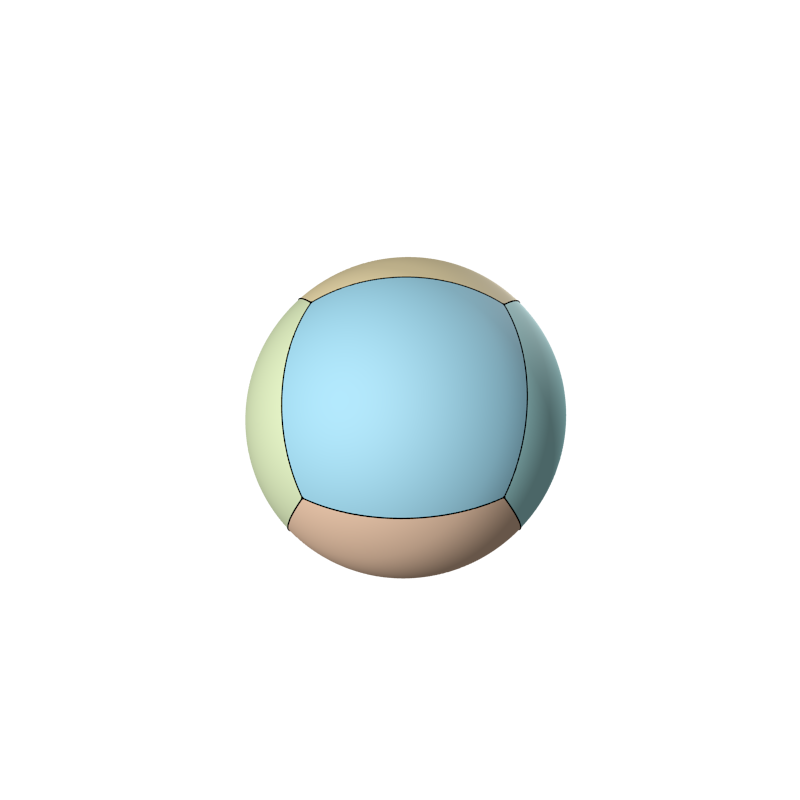
\includegraphics[width=\imagewidth]{vortex/snap_001}};
	\node[img] (im2) at (\imagewidth,         0) {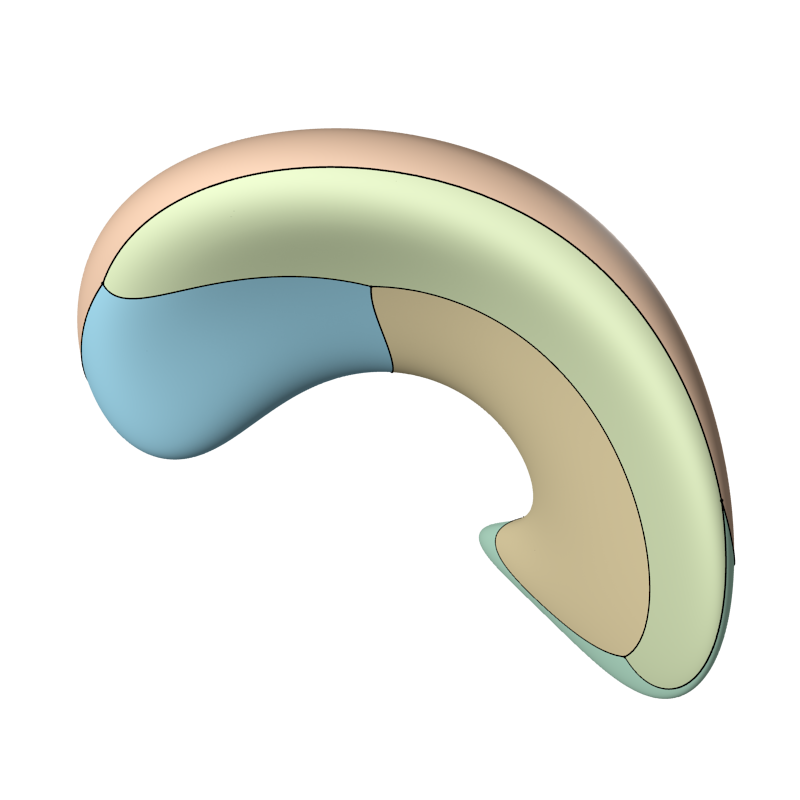
\includegraphics[width=\imagewidth]{vortex/snap_002}};
	\end{scope}%
	\node[img] (im3) at (          0,  -\imypos) {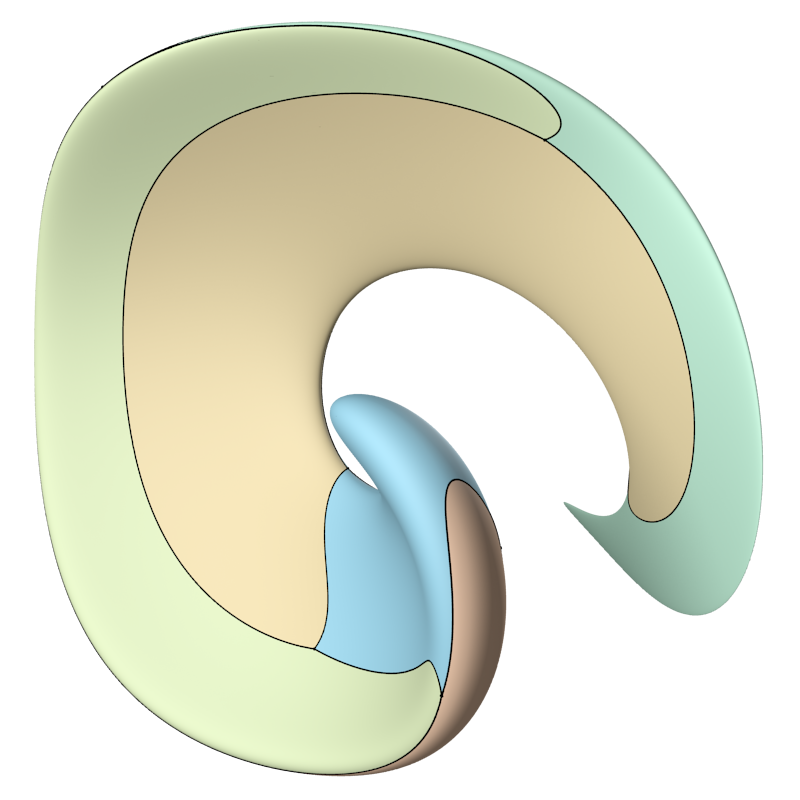
\includegraphics[width=\imagewidth]{vortex/snap_003}};
	\node[img] (im4) at (\imagewidth,  -\imypos) {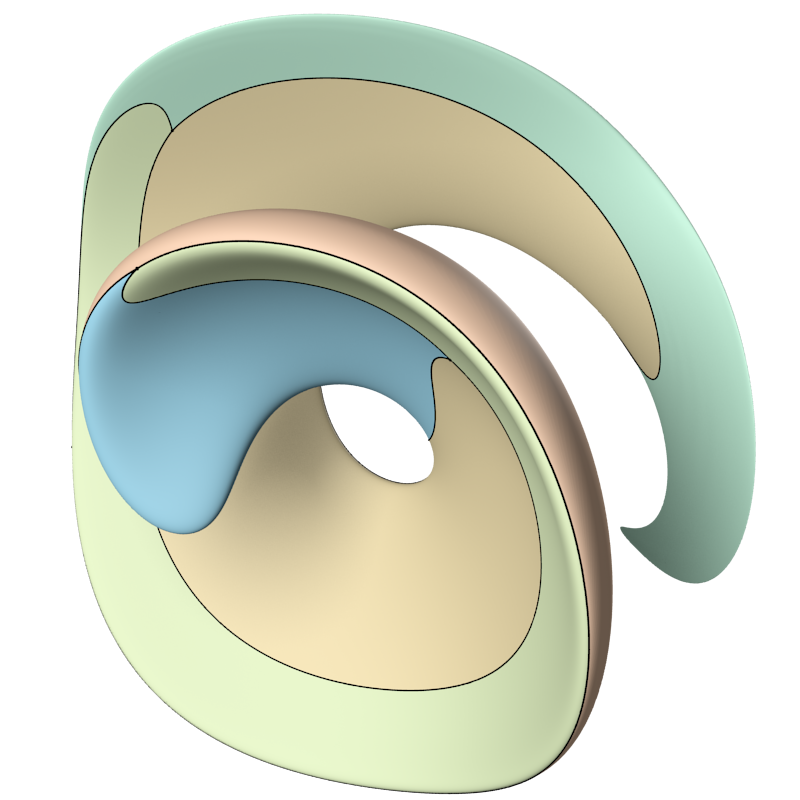
\includegraphics[width=\imagewidth]{vortex/snap_004}};
	\node[img] (im5) at (          0, -2\imypos) {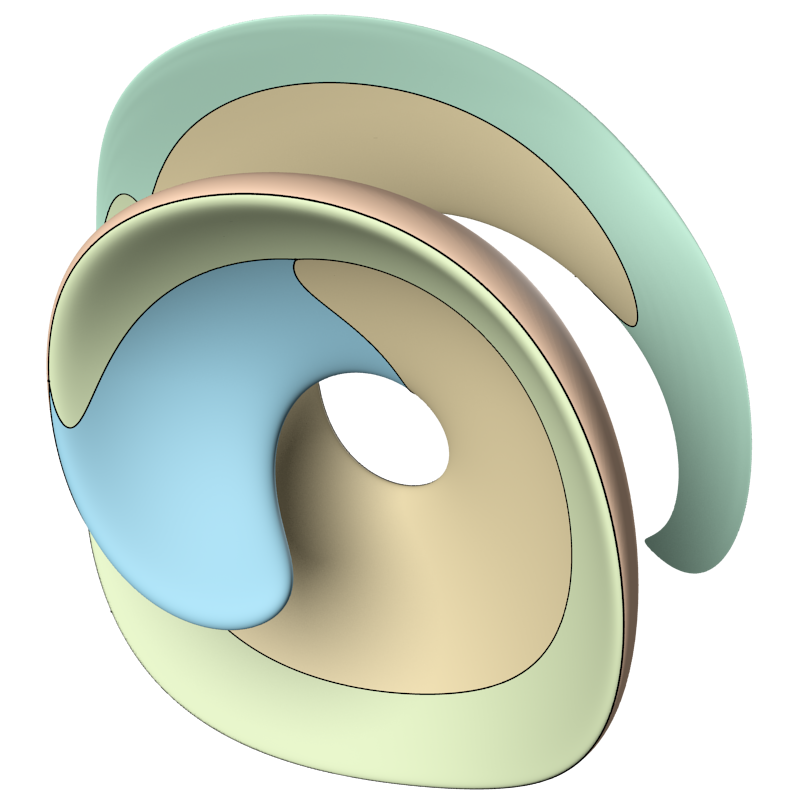
\includegraphics[width=\imagewidth]{vortex/snap_005}};
	\node[img] (im6) at (\imagewidth, -2\imypos) {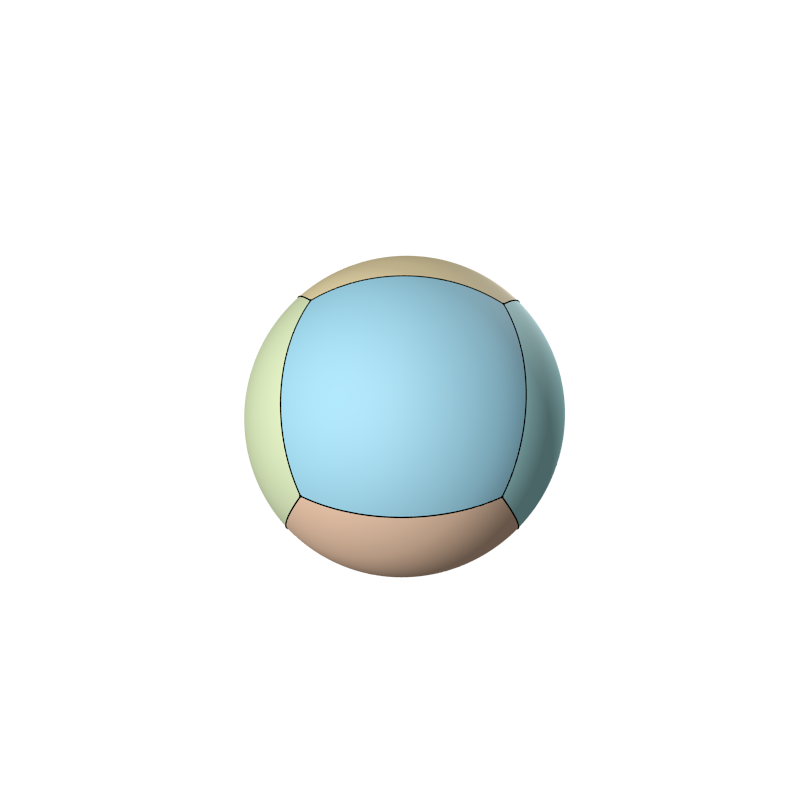
\includegraphics[width=\imagewidth]{vortex/snap_006}};
	%
	\node[txt] at (im1.south west) {$t=   0$};
    \node[txt] at (im2.south west) {$t= T/8$};
    \node[txt] at (im3.south west) {$t= T/4$};
    \node[txt] at (im4.south west) {$t=3T/8$};
    \node[txt] at (im5.south west) {$t= T/2$};
    \node[txt] at (im6.south west) {$t=   T$};
\end{tikzpicture}
	\caption{Aperçu du modèle \brep\ à différents instants de la déformation ($T=4$).}
	\label{fig:snapshots_vortex}
\end{figure}

paramétrisation : cube projeté sur sphère ou \guillemets{slerp}\\
calcul de volume avec quadrature de Clenshaw-Curtis (exact, l'intégrande est polynomiale) (étanchéité (continuité $\contgeom{0}$ partout) garantie car les marqueurs de bord coïncident tout au long de la déformation)\\
convergence de l'erreur d'approximation sur la position, l'aire et le volume à $t = 0$ et $t = T$ pour différents niveaux de discrétisations spatiale et temporelle\\

%%%%%%%%%%%%%%%%%%%%%%%%%%%%%
% FIGURES ERREUR VS DOF
\def\axw{0.48\textwidth}
\def\axh{0.39\textwidth}
\def\xlabl{$N$}%{$\mathrm{dof}$}
\def\ylabl{Erreur}
\def\xsep{2pt}
%%% POSITION
\plotVortexErrorVsDof{position}{la~}{pos}{maximale}
%%% AIRE
\plotVortexErrorVsDof{aire}{l'}{air}{relative}
%%% VOLUME
\plotVortexErrorVsDof{volume}{le~}{vol}{relative}
%%%%%%%%%%%%%%%%%%%%%%%%%%%%

+ convergence de la variation de volume au cours de la déformation (censée être nulle)\\
\begin{figure}
  \centering
  \begin{tikzpicture}%
  \begin{semilogyaxis}[%
    axis lines*=left,%
    width=9cm, height=7cm,%
    xmin = 0.0, xmax = 1.0,%
    ymin = 1e-16, ymax = 1e0,%
    ytickten = {-16,-12,-8,-4,0},%
    xtick distance=.25,
    grid=major,%
    xlabel={$t/T$},%
    ylabel={$\frac{\left|V - V_0\right|}{V_0}$},%
    legend style={font=\small, at={(0.5,0.033)}, anchor=south},%
    no marks, each nth point=1]%
    \pgfplotstableread{figures/data/vortex/vortex_erreur_volume_vs_time_0.001.dat}{\datatable}
    \pgfplotstablegetcolsof{\datatable}
    \pgfmathtruncatemacro\numberofcols{\pgfplotsretval-1}
    \pgfplotsinvokeforeach{1,...,\numberofcols}{%
		\pgfplotstablegetcolumnnamebyindex{#1}\of{\datatable}\to{\colname}%
		\addplot+ table [y index=#1] from \datatable;% node[right, pos=1, anchor=west] {$N = \colname$};%
		\addlegendentryexpanded{$N = \colname$}%
    }%
  \end{semilogyaxis}%
  \end{tikzpicture}%
  \caption{Évolution au cours du temps de l'erreur relative en volume pour différents niveaux de discrétisation spatiale. Le schéma de Runge-Kutta explicite à l'ordre 4 est utilisé pour l'intégration temporelle, avec un pas de temps $\Delta t = 0.001$.}
  \label{fig:vortex_error_volume_vs_time}
\end{figure}

Nuancer la pertinence d'un tel cas test :
\begin{itemize}
	\item pour d'autres cas test analogues (\eg Enright), un mouvement tangentiel des marqueurs lagrangiens est nécessaire (reparamétrisation)
	\item mais ce type de déformation extrême n'est pas celui que l'on vise dans nos applications, ce pourquoi on n'a pas trop considéré la reparamétrisation\ldots
	\item permet toutefois d'évaluer le pouvoir de résolution des polynômes de Chebyshev (vérifier la convergence rapide)
\end{itemize}

\section{Propagation à vitesse normale uniforme}
cube en expansion\par
intérêts :
\begin{itemize}
	\item valider l'approximation du vecteur normal
	\item valider la construction des EdS propres des arêtes et sommets convexes
\end{itemize}